\chapter{Eventmanagement}
\section{Einführung}
Events beziehungsweise Veranstaltungen sind in den letzten Jahren zu einem der bedeutendsten Marketinginstrumenten sowohl für Unternehmen, Organisationen als auch Privatpersonen aufgestiegen. Sie ermöglichen und fördern den Aufbau einer starken, persönlichen und emotionalen Beziehung zwischen den Veranstaltern und der dazugehörigen Kundenzielgruppe, was insgesamt zu einer besseren und dauerhafteren Kundenbindung führt. Ebenso bilden diese real Events einen kreativen Gegenpol zur voranschreitenden Digitalisierung, was durch die vermehrten virtuellen Konversationen und Begegnungen mit anderen Mitmenschen, Arbeitskollegen oder Stakeholdern von jedem einzelnen wahrgenommen werden kann.\autocite[Vgl.][]{Eventmanagementstudieren.de.o.J.}

Mit der globalen Ausbreitung des Covid-19 Virus mussten allerdings die meisten, wenn nicht sogar alle Events abgesagt oder auf unbestimmte Zeit verschoben werden, wie beispielsweise die Fußball Europameisterschaft 2020 oder auch die weltweit wichtigste sicherheitspolitische Konferenz, welche jährlich Anfang des Jahres in München stattfindet. 
Nur die allerwenigsten Veranstaltungen sind durch ein virtuell stattfindendes Event ersetzt worden, was auf die Notwendigkeit dieser einzelnen Veranstaltungen zurückzuführen ist, wie unteranderem der G7-Gipfel.\autocites[Vgl.][]{Tagesschau.o.J.}[Vgl.][]{Nahar.o.J.}

Das Eventmanagement beinhaltet alle notwendigen Aktivitäten für die erfolgreiche Durchführung eines Events. Es übernimmt also die Aufgaben der Zielsetzung, operativen Planung und Durchführung in einem vorgegebenen Rahmen. Im Eventmanagement steht stets der Kunde im Mittelpunkt, weshalb das Eventmanagement stark von subjektiven sowie psychologischen Aspekten geprägt ist.\autocite[Vgl.][]{ZeitOnline.o.J.}

\section{Begriff: Event}
Der Begriff \enquote{Event} hat seinen Ursprung im englischen Sprachraum und wird mit \enquote{Ereignis} oder auch \enquote{Veranstaltung} übersetzt. Aufgrund der stark subjektiven Wahrnehmung von Events gibt es in der Theorie und Praxis keine einheitliche und genaue Definition. Dennoch kann ein Event durch folgende zentrale Charakteristiken beschrieben werden: 

\begin{itemize}
    \item Erinnerungswert
    \item Einzigartig- und Einmaligkeit
    \item Aktivierung der Besucher, Positivität
    \item Planung, Organisation und Inszenierung
    \item erlebnisorientierten Ereignis
\end{itemize}

Mit diesem allgemeinen Verständnis von Events beziehungsweise Veranstaltungen soll nun die mögliche Kategorisierung von Events dargelegt werden. 

\begin{table}[!h]
    \centering
    \begin{tabular}{l|l}
        \textbf{Event-Cluster}      & \textbf{Beispiel} \\ \hline
        Kultur-Event                & Open-Air-Konzert, Festival, königliche Hochzeit        \\ \hline
        Sport-Event                 & Super-Bowl, Fußball-WM, Olympia   \\ \hline
        ökonomisches Event          & Apple Keynote, Hauptversammlung   \\ \hline
        politisches Event           & G7-, G20-Gipfel, Münchner Sicherheitskonferenz                   \\ \hline
        natürliches Event           & Sonnenfinsternis, Sternschnuppen        
    \end{tabular}%
    \caption{}
    \label{tab:event-cluster}
\end{table}

Eine dieser Systematisierungen besteht in der Unterteilung von Veranstaltungen basierend auf ihrer Größe. So klassifiziert der Autor Walter Freyer Events in Mega-, Medium- und Mikro-Events. Neben dieser einfachen Art der Systematisierung können Veranstaltungen aufgrund ihres Anlasses geclustert werden, wie in \autoref{tab:event-cluster} verdeutlicht. Eine Einheitliche Kategorisierung von Events gibt es aufgrund des subjektiven Aspekts erneut nicht. Deshalb wäre ebenso die Kategorisierung in Kommerzielle und Nicht-Kommerzielle Events eine korrekte Unterteilung von Events.\autocite[Vgl.][S. 23 ff.]{Eisermann.2014}

Ein Event wird aus einem bestimmten Grund geplant und durchgeführt. Deshalb sollte zu Beginn das Ziel bzw. der Zweck des Events festgehalten werden und während des gesamten Eventmanagementprozesses im Kopf behalten werden. Das jeweilige Ziel eines Events kann sehr unterschiedlich ausfallen und kann unter anderem sein:

\begin{itemize}
    \item Finanzieller Effekt
    \item Einfluss auf Personen
    \item Steigerung der Bekanntheit
    \item Akquirierung von Sponsoren und Teilnehmern
\end{itemize}

Von diesen primären Zielen eines Events lassen sich die sekundären Ziele ableiten. Mögliche sekundären Ziele sind eine hohe Besucherzahl oder auch eine starke Medienpräsenz. Insgesamt ist jedes Event am Ziel und folglich am Kunden / Besucher orientiert. Zum Erreichen dieses Ziels wird bei einem Event mit der Emotionalen Ebene gearbeitet, um die Teilnehmer zu erreichen. Deshalb ist ein Event stark subjektiv.\autocite[Vgl.][S. 6 ff.]{Holzbaur.2002}

\section{Aufgaben des Eventmanagement}
Das Eventmanagement umfasst alle Aufgaben der Planung, Organisation, Überwachung und Steuerung, die bei der Ausführung eines Events notwendig sind. Grundsätzlich wird ein Event wie ein Projekt geplant und durchgeführt, weshalb wesentliche Prinzipien des Projektmanagements ebenso im Eventmanagement beachtet werden müssen. Aus diesem Grund soll an dieser Stelle das magische Dreieck des Projektmanagements vorgestellt werden.\autocite[Vgl.][S. 22]{Holzbaur.2002}

Das magische Dreieck, dargestellt in \autoref{fig:EM_magisches_Dreieck}, besteht aus drei Ecken, die die drei Hauptmerkmale des Projekts repräsentieren:

\begin{figure}[H]
    \centering
    \setlength{\fboxsep}{10pt}
    \setlength{\fboxrule}{0.5pt}
    \fbox{
\includegraphics[width=0.65\textwidth]{img/EM_MagischesDreieck.png}}
    \caption[Eventmanagement: magisches Dreieck]{Darstellung des magischen Dreiecks aus dem Projektmanagements. (Quelle: In Anlehnung \autocite[]{Holzbaur.2002})} \label{fig:EM_magisches_Dreieck}
\end{figure}

\textbf{Ergebnis:} 
\\
Das Hauptmerkmal Ergebnis ist im Eventmanagement das Event selbst und stellt das oberste Ziel des Projektes dar. Wie bereits im oberen Abschnitt beschrieben lassen sich über das Event Sekundärziele ableiten. Beispielsweise ist das Primärziel die Veranstaltung eines Freundschaftsspiels zwischen einem großen und kleinen Fußballclub. Neben dem Sportereignis an sich, kann die Vorstellung eines Königstransfers oder das Aufbessern der Vereinskasse die Sekundärziele sein.

\textbf{Ressourcen:}
\\
Das Hauptmerkmal Ressourcen beinhaltet die monetären Mittel, die Infrastruktur wie Räumlichkeiten und Parkplätze sowie das Personal und Arbeitszeit. Die Ressourcen stellen also alle notwenigen Aufwendung während des gesamten Projekts dar.

\textbf{Zeit:}
\\
Das Hauptmerkmal Zeit oder im Eventmanagement Termin ist primär der Zeitpunkt der Ausführung des Events. Darüber hinaus zählt zu diesem Hauptmerkmal selbstverständlich auch das Einhalten von davor geplanten Terminen, wie unteranderem das rechtzeitige Plakatieren, versenden der Einladungen oder Verkauf von Event-Tickets.

Auch im Eventmanagement weisen die drei Hauptmerkmale Wechselwirkungen auf. So muss beispielsweise beim Ausfall von Personal während der Planung und Organisation des Events, das Hauptmerkmal der Zeit oder des Ergebnisses diese Veränderung im Hauptmerkmal der Ressourcen kompensieren. 

Aufgrund des Projektcharakters kann  ein Event in Meilensteine und Projektphasen unterteilt werden, wie in \autoref{fig:EM_PH_MS} veranschaulicht:

\begin{figure}[H]
    \centering
    \setlength{\fboxsep}{10pt}
    \setlength{\fboxrule}{0.5pt}
    \fbox{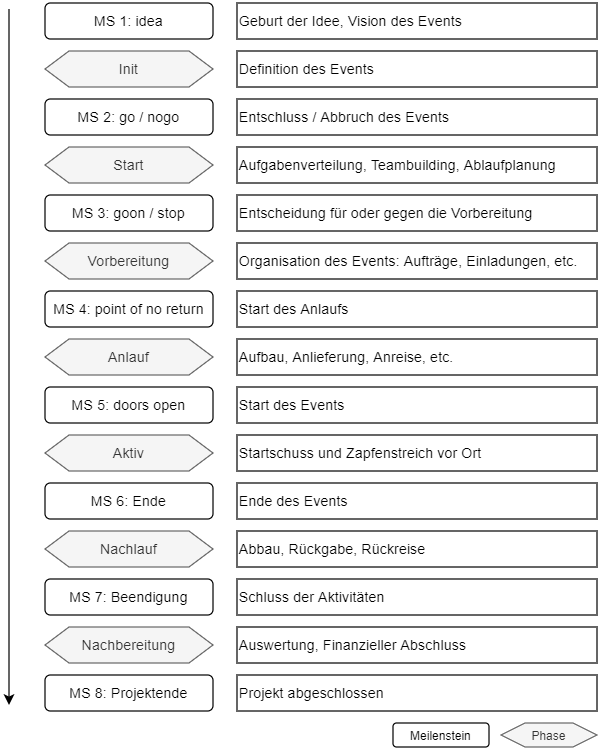
\includegraphics[width=0.7\textwidth]{img/EM_PH_MS.png}}
    \caption[Eventmanagement: Meilensteine und Phase eines Events]{Darstellung der acht Meilensteine und sieben Phasen bei der Veranstaltung eines Events. (Quelle: In Anlehnung \autocite[Vgl.][S. 23]{Holzbaur.2002})} \label{fig:EM_PH_MS}
\end{figure}

Die hier aufgezeigten Meilensteine und Phasen stehen in einer engen Beziehung zu einander und können gemeinsam als Grundlage eines Terminplans dienen. Die Termine und Dauer der jeweiligen Meilensteine und Phasen kann von Event zu Event stark variieren. Beispielsweise ist die Phase Aktiv eines Open-Air-Konzerts nur einige Stunden lang, wohingegen bei einem Musik-Festival diese Phase mehrere Tage dauert. Grundsätzlich leiten sich die Termine der Meilensteine von der Dauer den jeweiligen Phasen ab. Der Terminplan kann in einer einfachen Tabelle, Gantt-Diagramm oder ähnlichen Formen abgebildet werden.\autocite[Vgl.][S. 24 ff.]{Holzbaur.2002}

Neben der Gliederung eines Events in Meilensteinen und Phasen empfiehlt es sich zudem innerhalb des Projektes (Events) eine organisatorische sowie inhaltliche Struktur aufzubauen.

Die organisatorische Projektstruktur ist meist eine hierarchische Aufteilung in Aufgabenbereiche bzw. Teilprojekte. Mit dieser Aufteilung werden für verschiedene Bereiche Verantwortliche und Ansprechpartner sichergestellt. Eine grobe Projektorganisation innerhalb eines Events kann in \autoref{fig:EM_Aufbauorganisation} betrachtet werden. 

\begin{figure}[H]
    \centering
    \setlength{\fboxsep}{10pt}
    \setlength{\fboxrule}{0.5pt}
    \fbox{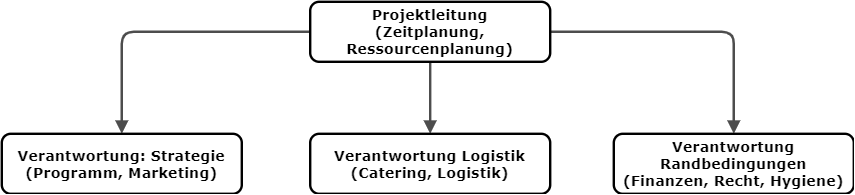
\includegraphics[width=0.8\textwidth]{img/EM_ORG.png}}
    \caption[Eventmanagement: Aufbauorganisation]{Darstellung einer High-Level Aufbauorganisation (Quelle: Eigene Darstellung} \label{fig:EM_Aufbauorganisation}
\end{figure}

Die inhaltliche Projektorganisation im Eventmanagement kann über den Projektstrukturplan PSP\autocite[]{projektmanagementdefinitionen.de.o.J.} erreicht werden. In diesem werden sämtliche Tätigkeiten eines Events aufgenommen. Tätigkeiten stellen dabei die kleinste Arbeitseinheit dar. Mehrere Tätigkeiten können wiederum zu einem Arbeitspaket zusammengefasst werden und Arbeitspakete können letztlich zu Teilprojekte zusammengefasst werden.\autocite[Vgl.][S. 144 f.]{Holzbaur.2002}

Mit Hilfe des Strukturplans erhalten die Verantwortlichen eine bessere Übersicht über die einzelnen Aufgaben und Arbeitspakete. Zudem unterstützt der Strukturplan den Projektleiter bei Controlling spezifischen Aufgaben.

Nachdem ein grober Überblick über die Projektstruktur sowie Meilensteine und Eventphasen gegeben worden ist soll nun die verschiedenen Aufgabenbereiche innerhalb eines Events genauer betrachtet werden. Wie bereits in Abbildung dargelegt können drei Hauptaufgabenbereiche ausgemacht werden: Strategie, Logistik und Randbedingungen. 

\textbf{Strategie:}

Der Aufgabenbereich der Strategie befasst sich mit den Themen Marketing und Programm. Die Kernaufgabe besteht in der Zieldefinition des Events. Nachdem dieses Ziel festgelegte wurde muss anschließend ein passendes Eventprogramm entwickelt werden. Hierfür muss eine Zielgruppe definiert werden und eine sorgfältige Analyse des Markts durchgeführt werden, um ein erfolgreiches Programm zu entwerfen. Ein mögliches Eventprogramm wird in einem folge Kapitel vorgestellt. Neben der Erstellung des Eventprogramms ist eine weitere wesentliche Aufgabe die Ausarbeitung einer passenden Marketingkampagne. Beispiele solcher Marketingmaßnahmen sind Werbevideos oder auch Broschüren. Allerdings müssen je nach Event und Zielgruppe entsprechende Kommunikationswege ausgewählt werden. Die letzte wesentliche Aufgabe dieses Bereichs besteht in der Suche nach einem möglichen Sponsoring. Diese Aufgabe kann allerdings je nach Event entfallen.

\textbf{Logistik:}

Der Aufgabenbereich der Logistik beinhaltet alle Tätigkeiten, die einen reibungslosen Ablauf eines Events sicherstellt. Die erste und wichtigste Aufgabe besteht in der Festlegung der Eventlocation. Diese muss selbstverständlich abhängig des Eventziels und Eventgröße ausgewählt werden. Des Weiteren organisiert der Aufgabenbereich der Logistik das Catering, die Aufteilung der Räumlichkeiten und für eine eventuelle Bereitstellung von Transportmöglichkeiten wie beispielsweise vom Flughafen zur Eventlocation. Auch die Müllentsorgung ist Teilaufgabe dieses Aufgabenbereichs und sollte bei der Planung eines Events nicht unberücksichtigt bleiben.

\textbf{Randbedingungen:}

Der Aufgabenberiech der Randbedingungen hat drei Hauptaufgaben. Die erste dieser besteht in der rechtlichen Absicherung. Beispielsweise können Genehmigung der Stadt notwendig sein, um ein Event an einem Sonntag ausführen zu dürfen. Die zweite Aufgabe besteht in der Ausarbeitung eines Sicherheits- sowie Gesundheitskonzepts. Sowohl die Sicherheit als auch Gesundheit muss während eines Events sichergestellt werden. Durch die Entwicklungen in den letzten Jahren durch verschiedene Attentate aber auch durch Corona-Pandemie steigt die Wichtigkeit dieser beiden Aspekte. Durch die Ausarbeitung solcher Konzepte kann in Notsituationen auf diese zurückgegriffen werden und möglicherweise schlimmeres verhindern. Die dritte Hauptaufgabe besteht in der Überwachung der Finanzen und Wirtschaftlichkeit des Events, wie beispielsweise die Buchführung.

Neben diesen drei Aufgabenbereichen kann auch das Projektmanagement als solches gewertet werden. Allerdings würde eine ausführliche Erläuterung der Aufgaben des Projektmanagements den Rahmen dieser Arbeit sprengen, weshalb auf eine genauere Ausarbeitung verzichtet wird und auf die zahlreiche Literatur, die dieses Thema behandelt, hingewiesen.
